%TODO: colocar especificações
% -----------------------------------------------------------------
% => RESULTADOS
% -----------------------------------------------------------------
\label{chapter:resultados}

Essa seção descreve o planejamento, projeto, execução e análise dos resultados de um estudo experimental para avaliar o método proposto neste trabalho quando aplicado 
em \textit{benchmark} públicos de programas em GNU-C ou ANSI-C. 

% -----------------------------------------------------------------
% => Planejamento e projeto dos experimentos
% -----------------------------------------------------------------
\section{Planejamento e projeto dos experimentos}
\label{sub:experimento}

Esta avaliação experimental visa avaliar a habilidade do Map2Check com LLVM em gerar e verificar casos de testes (assertivas) relacionados a gerência de memória, especificamente desalocações inválidas de memória. 
Neste sentido, foi definido as seguintes questões de pesquisa:
\begin{description}
\item[QP1:] Os casos de teste gerados pelo Map2Check são suficiente para identificação de uma desalocação inválida do programa analisado?
%
\item[QP2:] Qual a eficácia do Map2Check para detectar falhas de desalocações inválidas quando comparado com outras ferramentas?
%
\item[QP3:] O método proposto aprimora a detecção de falhas de desalocações inválidas quando comparado a versão anterior do Map2Check?
\end{description}

Visando responder essas questões, foram utilizados $14$ programas da categoria 
\textit{MemorySafety} do \textit{benchmark} da \textit{Competition on Software Verification} (SV-COMP) \cite{beyer:2016}. Estes programas são classificados com \texttt{FALSE(valid-free)}, ou seja, esses programas contém desalocação inválida de memória. O SV-COMP é uma competição internacional onde diversas ferramentas são submetidas a \textit{benchmark} públicos (obtidos de diferentes domínios como \textit{drivers} e \textit{kernel} do Linux) e depois avaliadas e pontuadas. Assim, o SV-COMP tem como objetivo avaliar a transferência de tecnologia e comparar verificadores de software no estado da arte em relação à eficácia e eficiência. 
%Na categoria \textit{MemorySafety} foram pegos os 

\par
Nos \textit{benchmarks} da SV-COMP, alguns programas adotam funções específicas, por exemplo, a categoria de \textit{MemorySafety} contém a função \texttt{\_\_VERIFIER\_nondet\_int} que modela valores não determinísticos de inteiros. No Map2Check, foi implementado uma instrumentação para que o Klee (utilizando execução simbólica) gere os valores necessários para explorar os caminhos de execução do programa e então efetuar a verificação das assertiva nos  programas analisados.

\par
A execução da ferramenta Map2Check para avaliar os \textit{benchmarks} foi feita utilizando a ferramenta Benchexec \cite{beyer:2015} que gerencia, monitora e faz medidas de recursos (memória e tempo de execução pela CPU) utilizados por ferramentas. 
%
No Benchexec foram adotas as seguintes configurações para execução do experimento: 
um tempo máximo de execução (\textit{timeout}) de 15 minutos por programa a ser analisado, ou seja, se o Map2Check não chegar a uma conclusão dentro desse tempo, a execução será interrompida; 
%para aquela entrada e a próxima será executada (e o resultado do teste será uma indeterminação). 
$8$ GB de memória RAM; e 
$5$ núcleos de processador.  
A máquina utilizada para execução do experimento continha um sistemas operacional Linux Ubuntu $16.10$ com $16$GB de memória, processador AMD $2.9$ GHz com $8$ cores de CPU. 
%
%Antes da execução já se sabia que no momento atual a implementação atual do Map2Check não %suporta \textit{loops} e o Klee pode gerar muitos valores simbólicos causando ocupação de um %espaço muito grande de memória. Então o foco da análise foi em verificar a quantidade de %falsos positivos e de falsos negativos que a ferramenta geraria.

\par
A avaliação foi conduzida da seguinte forma: 
(1) Aplicação do Map2Check sobre os programas do \textit{benchmark} do SV-COMP; 
(2) Comparação dos resultados obtidos (diretamento da página oficial do SV-COMP) com a versão anterior do Map2Check\footnote{https://sv-comp.sosy-lab.org/2016/results/results-verified/META\_Heap.table.html} \cite{beyer:2016}, ESBMC e Symbiotic 4\footnote{https://sv-comp.sosy-lab.org/2017/results/results-verified/META\_MemSafety.table.html}. 
Vale ressaltar que nos resultados da versão anterior do Map2Check no SV-COMP de 2016 havia um programa a menos na categoria \textit{MemorySafety}.

% -----------------------------------------------------------------
% => Execução dos experimento e Análise dos Resultados
% -----------------------------------------------------------------
\section{Execução dos experimento e Análise dos Resultados}

Após a execução dos \textit{benchmarks}, foram obtidos os resultados mostrados na \autoref{tabela:resultados}, onde cada linha da tabela contém: 
(1) nome da ferramenta (Ferramenta); 
(2) número de programas que a ferramenta identificou corretamente (Corretos); 
(3) número de programas que a ferramenta identificou um erro para um programa que atende todas as especificações (Falsos Negativo); 
(4) número de programas em que a ferramenta falhou para computar a verificação (Desconhecidos); e 
(5) número de programas avaliados (Total).

\begin{table}[H]
	\caption{\label{tabela:resultados} Resultado da experimentação}
	\begin{center}
	    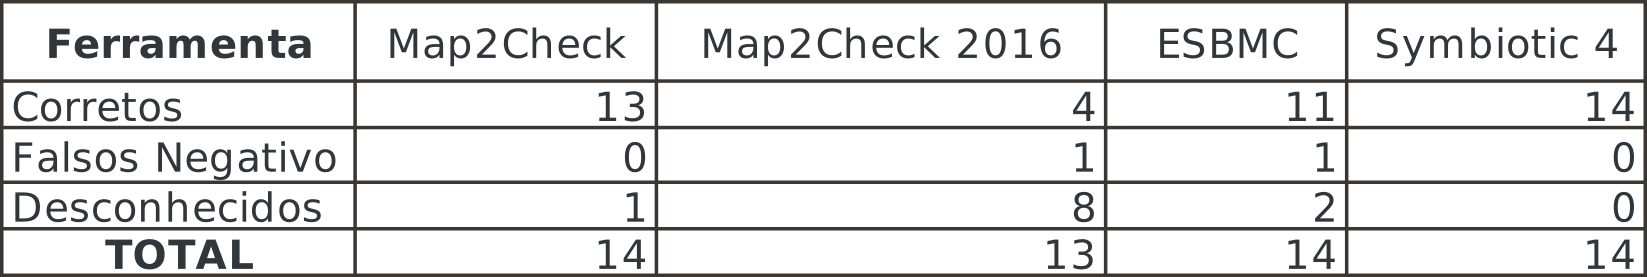
\includegraphics[scale=0.33]{resources/tabelaResultados.png}
	\end{center}
	\legend{Fonte: Própria}
\end{table}

Para respondermos a questão de pesquisa \textbf{QP1} e \textbf{QP2} da \autoref{sub:experimento}, foi analisado a \autoref{tabela:resultados} que mostra que o Map2Check classificou corretamente aproximadamente $93\%$ dos programas avaliados, enquanto o Simbiotic $4$  classificou corretamente  $100$\%, o ESBMC classificou corretamente  aproximadamente $79$\%. O Map2Check não gerou nenhum falso positivo nem falso negativo, foi gerado apenas um resultado desconhecido, acredita-se que é um caso de melhorias para a execução simbólica, por exemplo, por meio da aplicação de um \textit{slicer} de código \cite{Chalupa:2016}. 
%foi pela não utilização de um \textit{model checker}. %
No futuro, é planejado adotar um \textit{slicer}, bem como, um \textit{model checker} para ampliar o conjunto de propriedades inferidas, como é apresentado na \autoref{sec:cronograma}. 

\par
Com respeito  a questão de pesquisa \textbf{QP3} da \autoref{sub:experimento}, utilizando \autoref{tabela:resultados} podemos comparar os resultados, visando uma comparação mais justa, foi excluído o programa que a versão anterior do Map2Check não analisou e como a versão atual categorizou esse programa de forma correta, vamos subtrair 1 do total de corretos. A nova versão do Map2Check então classificou corretamente 92\% dos casos e a versão antiga 31\%. A versão antiga havia gerado um falso negativo enquanto a nova não gerou nenhum.
%\par
Os resultados, embora preliminares em natureza, sugerem fortemente que o método pode ser eficaz em gerar e validar casos de teste para verificação de desalocações inválidas de programas em C. Vale ressaltar que novos experimentos serão realizados a fim de determinar a eficácia da nova versão do Map2Check com LLVM.

%Então, pode-se defender de que o Map2Check integra teste e verificação. O teste é baseado é %análise dinâmica e verificação de assertivas. As assertivas contém um conjunto de %especificações.